\section{Planning Initial}
Après avoir défini les objectifs, leur avoir donné une complexité et une business
value, nous avons pu créer un planning prévisionnel, basé sur un diagramme de Gantt. Pour
trier les objectifs chronologiquement nous avons défini une valeur "Sprint complexity"
égale à la complexité sur la business value. L'ordre croissant nous a donné l'ordre
chronologique. Il a tout de même fallu modifier cet ordre en tenant compte des dépendances
entre certains objectifs. Finalement, nous avons découpé le temps global du projet en 6
sprints, correspondant à l'écart entre chaque revue de projet. Nous avons donc élaboré le
diagramme de Gantt présenté en Figure \ref{gantt}.

\begin{figure}
    \center
    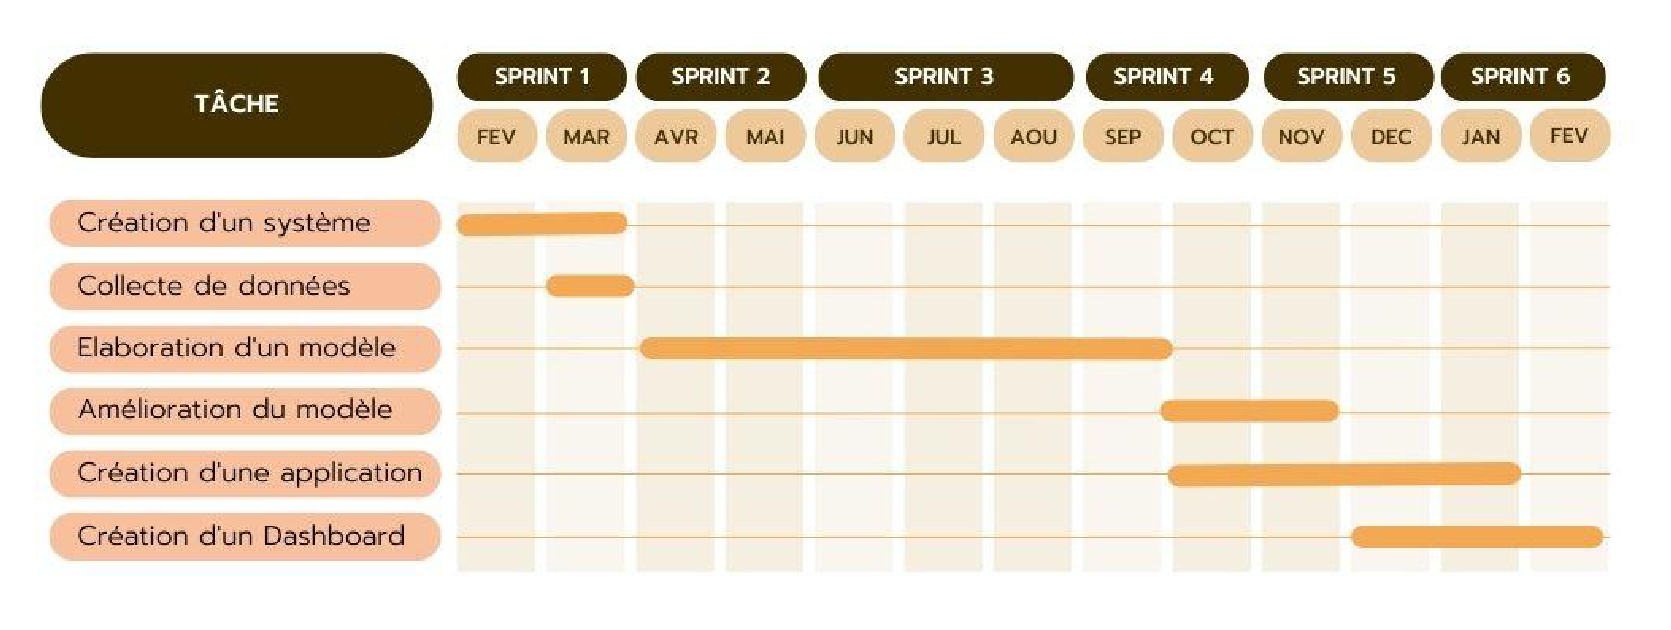
\includegraphics[scale=.2]{img/gantt.png}
    \caption{Planning initial (Diagramme de Gantt)}
    \label{gantt}
\end{figure}